\documentclass[../../main.tex]{subfiles}

\begin{document}

\subsection{Analyse}\label{sec:analyse}
I UP går aktiviteten analyse ud på, at afdække forretningesområdet. Analysen kan ses fra to view's: Et statisk view, som inbefatter analyseklasser og analysediagram, og et dynamisk view som inbefatter interaktionsdiagrammer, udledt ved brugsmønsterrealisering. I det statiske view ses systemets overordnede opbygning, altså systemet i stilstand, hvor man i det dynamiske view ser et øjebliksbillede af systemet i brug. 

\paragraph{Statiske view} \mbox{} \\
Analysemodellen for systemet ses på figur \ref{fig:analysemodel}. Her ses det, at systemet er analyseret til, at der skal være to pakker i domain-laget; \code{sikkerhed} og \code{udredning}. Dette er gjort for at adskille sikkerheden i systemet fra udredningen, så begge pakker nemt kan udskiftes. Sikkerhedspakken er opbygget ved, at der er en bruger, som har loginoplysninger. Hver bruger har en rolle, som beskriver hvad brugeren kan i systemet. Som led i analysearbejdet blev GDPR overvejet. Det betyder blandt andet, at personlige oplysninger omkring brugeren skal holdes adskilt. Det er derfor brugeren kun har login oplysninger, og at der i udrednings-pakken er en person-klasse, som indholder en persons navn og andre oplysninger. Slutteligt har klassen \code{Borger} CPR-nummer, der altså er adskilt fra både bruger og person i systemet, og derved også i databasen. 

\begin{figure}[H]
  \centering
  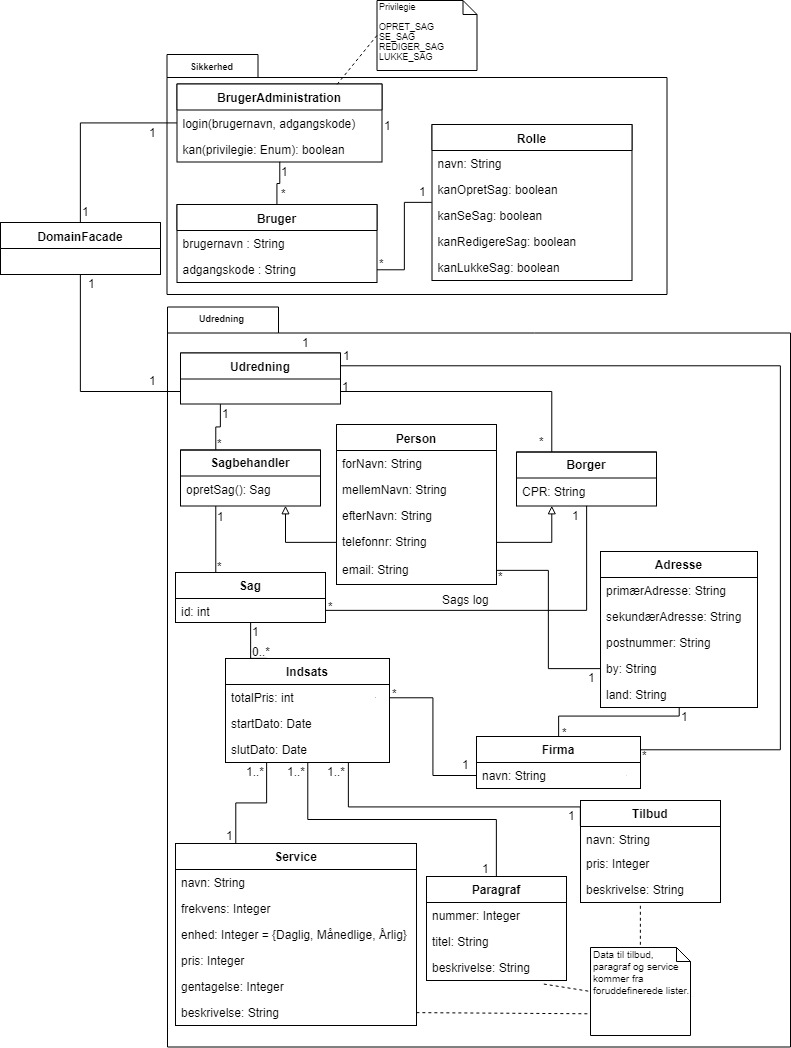
\includegraphics[scale=.38]{figurer/analysemodel.jpg}
  \caption{Analyseklassediagram}
  \label{fig:analysemodel}
\end{figure}

Analysemodellen består af analyseklasser. Figur \ref{fig:analyseklasse} viser analyseklassen \code{BrugerAdministration}. Denne klasse fungerer som en facadeklasse til sikkerhedspakken, hvorfra klassens navn kommer, da det beskriver klassens hensigt. Sikkerheden i systemet består af to centrale tjenester; at logge ind, og at tjekke om den nuværende bruger har privilegie til at udføre en handling. Derfor ligger disse tjenester på \code{BrugerAdministration}, da de skaber en høj samhørighed og en lav kobling. At finde de rette analyseklasser er en meget vigtig process for udviklingen af et system, da resten af udviklings processen ellers ødelægges. En god analyseklasse beskriver klart et koncept fra virkeligheden. Dette afspejler \code{BrugerAdministration}.

\begin{figure}[H]
  \centering
  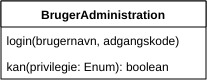
\includegraphics[scale=.5]{figurer/BA.jpg}
  \caption{Analyseklasse: BrugerAdministration}
  \label{fig:analyseklasse}
\end{figure}

\paragraph{Dynamiske view} \mbox{} \\
Brugsmønsterrealiseringen laves til de brugsmønstre der arbejdes med i den nuværende iteration. Processen består af fire dele. Der blev lavet brugsmønsterrealisering for to brugsmønstre: Sagsåbning og Login. Det første punkt i realiseringen er, at lave system interaktions diagrammer for brugsmønsteret, der skal realiseres. Denne process er udført på de to brugsmønstre der er fokus på i projektet. På figur \ref{fig:si:login} ses system interaktionsdiagrammet for login. Det er kendetegnende for et system interaktionsdiagram, at systemet er vist som en black box. Dette vil sige at det kun er de eksterne events der ses, og ikke de interne events i systemet. Det er også vigtigt at lægge mærke til, at der vises et "happy day scenario" over brugsmønstret. Der tages altså ikke højde for eventuele fejlkilder. Det første event, \code{login()}, sker når brugeren prøver at logge ind i systemet.   

\begin{figure}[H]
  \centering
  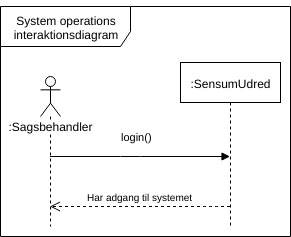
\includegraphics[scale=.6]{figurer/Login.jpg}
  \caption{System interaktionsdiagram: Login}
  \label{fig:si:login}
\end{figure}

Figur \ref{fig:sags_aabning_interaktion} viser brugernes interaktion med systemet, når en ny sag skal oprettes. Brugeren trigger eventet \code{åbenSag()}, som opretter en sag i systemt som skal udfyldes. Før sagen oprettes tjekkes der, om brugen har privilegie til at oprette sagen. Herefter indtaster brugeren oplysninger i sagen. Når brugeren ønsker at gemme sagen, trigger brugeren eventet \code{gem()}, som gemmer sagen persistent.

\begin{figure}[H]
  \centering
  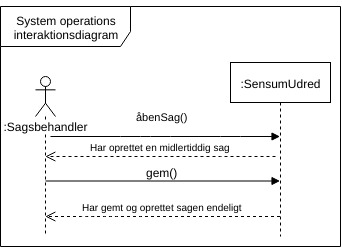
\includegraphics[scale=.6]{figurer/Sags_aabning_interaktion.jpg}
  \caption{Systeminteraktionsdiagram over hændelsesforløb for sagsåbbning brugsmønsteret}
  \label{fig:sags_aabning_interaktion}
\end{figure}

Det næste der skal ske i realiseringen er, at lave system operations kontrakter. Disse kontrakter beskriver hvad der sker som følge af en operation, og ikke hvad der sker under operationen. Den føste kontrakt, tab \ref{tab:kon:login}, beskriver \code{Login()} ansvarsområde. Den skal oprette en bruger hvis loginoplysningerne er korrekte. Kontrakten sammenlagt med analyseklassen på figur \ref{fig:analyseklasse} viser klassernes ansvarsfordeling, som indbefatter at en klasse kan vide noget og gøre noget. Her ved \code{BrugerAdministrator} hvem den nuværende bruger er, og den er i stand til at logge en bruger ind og tjekke hvad brugeren kan i systemet. 

\begin{table}[H]
\centering
\footnotesize
\resizebox{0.9 \textwidth}{!}{%
\begin{tabular}{| p{1\textwidth} |} \hline
\textbf{Kontrakt} \\ \hline

\textbf{Operation}  \\
login(username, password) \\ \hline

\textbf{Krydsreference} \\
Login\\ \hline

\textbf{Ansvar} \\
  \begin{minipage}[t]{\textwidth}
    \begin{itemize}
    \item[-] For at instanitiere en bruger, hvis autentificerings-oplysningerne er korrekte:
    \begin{itemize}
    	\item[-] Autentificerings-oplysningerne er korrekte hvis password og username passer med oplysninger i systemet.
    \end{itemize}
    \end{itemize}
  \end{minipage}
\\ \hline

\textbf{Output} \\
Ingen  \\ \hline

\textbf{Prækonditioner} \\
  \begin{minipage}[t]{\textwidth}
    \begin{itemize}
    \item[-] Må ikke være logget ind i forvejen. 
    \end{itemize}
  \end{minipage} \\ \hline

\textbf{Postkonditioner} \\
  \begin{minipage}[t]{\textwidth}
    \begin{enumerate}
    \item[-] Der er oprettet en instans af sagsbehandleren.
    \end{enumerate}
  \end{minipage} \\ \hline
 
\end{tabular}}
\caption{Kontrakt over Login brugsmønsteret}
\label{tab:kon:login}
\end{table}

De næste to kontrakter omhandler sagsåbningen, hvor de to centrale operationer er \code{open}, tab \ref{tab:kon:openCase}, og \code{save}, tab \ref{tab:kon:saveCase}. \code{Open} har ansvaret for at oprette en ny sag og returnere den til sagsbehandleren, så den kan redigeres i. \code{save} har ansvar for at gemme sagen persistent. Begge disse kontrakter har som prækondition, at brugeren skal være logget ind og have rettigheder til at udføre handlingen, da det er vigtigt at det kun er brugere der har rettigheder til det, der kan udføre handlingerne.

\begin{table}[H]
\centering
\footnotesize
\resizebox{0.9 \textwidth}{!}{%
\begin{tabular}{| p{1\textwidth} |} \hline
\textbf{Kontrakt} \\ \hline

\textbf{Operation}  \\
open() \\ \hline

\textbf{Krydsreference} \\
Sagsåbning
      \\ \hline

\textbf{Ansvar} \\
  \begin{minipage}[t]{\textwidth}
    \begin{itemize}
    \item[-] For at instanitiere en tom sag, hvis den aktuelle sagsbehandler har tilladelse.
	\item[-] At returnere en sag, så den kan blive udfyldt.
    \end{itemize}
  \end{minipage}
\\ \hline

\textbf{Output} \\
Ingen  \\ \hline

\textbf{Prækonditioner} \\
  \begin{minipage}[t]{\textwidth}
    \begin{itemize}
    \item[-] En sagsbehandler er logget ind. 
    \item[-] Sagsbehandleren har rettigheder til at udfører handlingen.
    \end{itemize}
  \end{minipage} \\ \hline

\textbf{Postkonditioner} \\
  \begin{minipage}[t]{\textwidth}
    \begin{enumerate}
    \item[-] Der er oprettet en instance af sag. 
    \end{enumerate}
  \end{minipage} \\ \hline
 
\end{tabular}}
\caption{Kontrakt over åben sag}
\label{tab:kon:openCase}
\end{table}

\begin{table}[H]
\centering
\footnotesize
\resizebox{0.9 \textwidth}{!}{%
\begin{tabular}{| p{1\textwidth} |} \hline
\textbf{Kontrakt} \\ \hline

\textbf{Operation}  \\
save() \\ \hline

\textbf{Krydsreference} \\
Sagsåbning
      \\ \hline

\textbf{Ansvar} \\
  \begin{minipage}[t]{\textwidth}
    \begin{itemize}
    \item[-] For at gemme en sag, hvis den aktuelle sagsbehandler har tilladelse.
	\item[-] At returnere om sagen er gemt.
    \end{itemize}
  \end{minipage}
\\ \hline

\textbf{Output} \\
Ingen  \\ \hline

\textbf{Prækonditioner} \\
  \begin{minipage}[t]{\textwidth}
    \begin{itemize}
    \item[-] En sagsbehandler er logget ind. 
    \item[-] sagsbehandleren har rettigheder til at udføre handlingen.
    \item[-] En sag er oprettet og udfyldt.
    \end{itemize}
  \end{minipage} \\ \hline

\textbf{Postkonditioner} \\
  \begin{minipage}[t]{\textwidth}
    \begin{enumerate}
    \item[-] Sagen er gemt persistent. 
    \item[-] Sagsbehandleren har fået svar på om sagen er gemt.
    \end{enumerate}
  \end{minipage} \\ \hline
 
\end{tabular}}
\caption{Kontrakt over gem sag}
\label{tab:kon:saveCase}
\end{table}

Næste trin er, at uddelegere ansvar til de forskellige analyseklasser. Til at gøre dette, er der blevet brugt GRASP (General Responsibility Asssignment Software Patterns) patterns. Der blev analyseret frem til, at sikkkerheds- og systempakken havde brug for en controller. Så \code{AuthManager} og \code{System} fungerer som controller. De fungerer som facadeklasser til den overordnede facade \code{DomainFacade}. Et sted hvor det var mere udfordrende at tildele ansvaret, var i hvorhold til hvem der har ansvar for at oprette en ny sag. Her er både borgerne og sagsbehandleren kandidater. Borgeren kan ses som en information expert, da borger-klassen besidder en masse information, som skal bruges til at udfylde en sag. Samtidig kan sagsbehandleren ses som en Creator, da sagsbehandleren er den der interagerer direkte med sagen. Det er i systemet valgt at det er sagsbehandleren der har ansvaret for at oprette en sag. 

Det fjerde og sidste trin i realiseringen er, at opdatere analyseklassediagrammet ud fra \\
brugsmønsterrealiseringen. Processen viser her sin itterative natur, i og med at det opfordres til at returnere til tidligere resultater, og opdatere og ændre i disse. Analysediagrammet, set tidligere på figur \ref{fig:analysemodel}, er det endelige diagram. 

\end{document}